\chapter{Related Work}
\label{chapter:related}

A common source of realistic synthetic data is found in video games. We discuss the use of video games for this purpose in Section \ref{sec:video-games}.

\section{Synthetic Data Generation with Video Games and Other Software}
\label{sec:video-games}


Video games present the lowest barrier of entry in the domain of synthetic video data generation. This is because they combine realistic graphics meant to suspend human disbelief with high-performance rendering engines that achieve fast render times in large resolutions, on commodity hardware.

\begin{figure}[H]
    \centering
    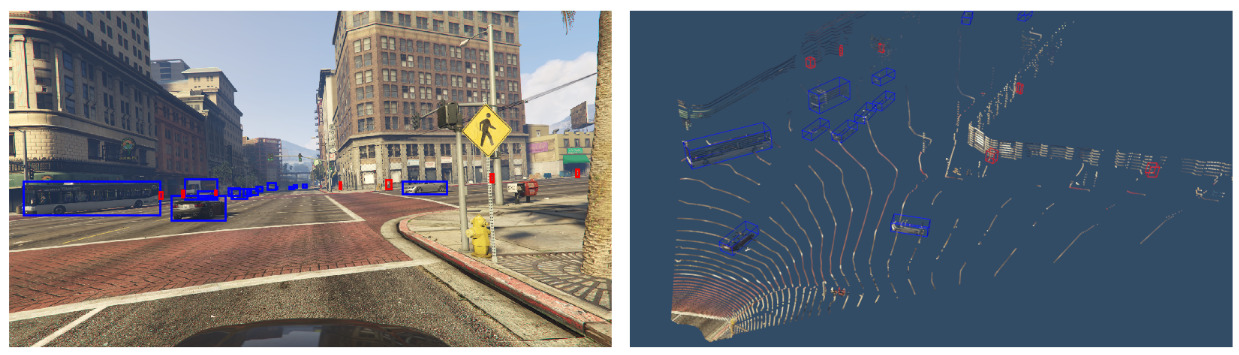
\includegraphics[width=\textwidth]{src/img/reated-pics/gta5-poza.jpg}
    \caption{LIDAR Simulation using GTA V\cite{hurl2019precise}}
    \label{fig:relatex-example-gta5}
\end{figure}

The most popular video game platform for generating synthetic video for deep learning datasets is, by far, "GTA V" by Rockstar Games. This platform was used for semantic segmentation\cite{richter2016playing}, LIDAR simulation \cite{hurl2019precise}, crowd counting \cite{wang2019learning}, and pedestrian detection and tracking\cite{Fabbri_2021_ICCV}. Other off-the-shelf software programs have also been used for image tasks, such as Google Earth \cite{marcu2018safeuav}.


\begin{figure}[H]
    \centering
    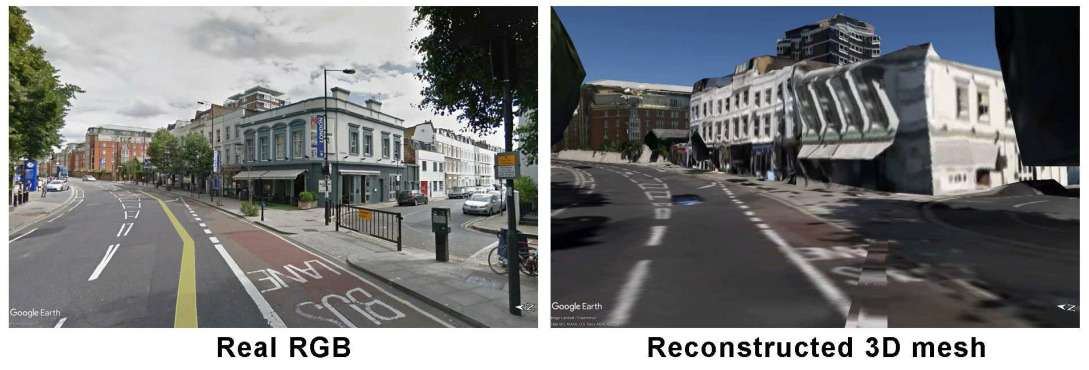
\includegraphics[width=\textwidth]{src/img/reated-pics/goog-earth.jpg}
    \caption{Synthetic Aerial 3D Dataset Generation using Google Earth\cite{marcu2018safeuav}}
    \label{fig:relatex-example-gta5}
\end{figure}

Using video games for this task, however, has a number of disadvantages. Firstly, all video games have a specific artistic style in their renditions of reality, which becomes another task that must be solved: domain adaptation \cite{wu2019squeezesegv2,wang2019learning}. Other issues include lack of control in the simulation, inability to add or edit models and environments, and a need to reverse-engineer proprietary, closed source software. This led to the development of specialized software meant to extract data from specific games \cite{doan2018g2d}.

An alternative to closed-source programs and video games is the use of game engines. These afford the user complete control over what, and how, is being rendered. We discuss the use of game engines for synthetic video generation tasks in the next section.

\section{Synthetic Data Generation with Game Engines}
\label{sec:graphics-engines}

Game engines are software frameworks meant to design and implement video games. As such, they give the user total control over how the simulation renders and runs. Popular game engines used for synthetic dataset generation include the proprietary Unity\footnote{\url{https://unity.com/}} and Unreal\footnote{\url{https://www.unrealengine.com/en-US}} engines, as well as the open-source project Blender\footnote{\url{https://www.blender.org/}}.


\begin{wrapfigure}{r}{0.5\textwidth}
    \centering
    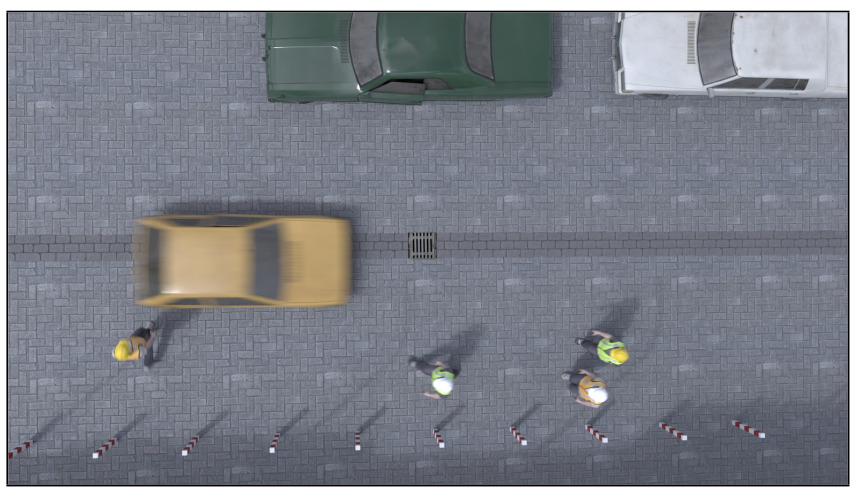
\includegraphics[width=0.48\textwidth]{src/img/reated-pics/construction-worker-tracking.jpg}
    \caption{Synthetic scenes for tracking construction workers using Blender\cite{neuhausen2020using}}
    \label{fig:relatex-example-construction-workers}
\end{wrapfigure}


Applications of game engines in synthetic video dataset generation include UAV monitoring and detection \cite{barisic2022sim2air}, procedural urban and outdoor environments \cite{ros2016synthia,khan2019procsy,stein2018genesis}, and indoor environments \cite{martinez2021unrealrox+}. Applications include tracking construction workers\cite{neuhausen2020using}, self-driving car obstacle avoidance\cite{bhandari2018procedural,pouyanfar2019roads}, or more generally rendering generic environments with people\cite{kerim2021nova}.

Of the more general-use projects that build upon game engines, we bring attention to Kubric \cite{greff2021kubric}, a project concerned with realism, scalability and flexibility.

Since a scene is only as complex as its included 3D assets, the data diversity generated by game engines with static assets is limited in scope. To create the large variance needed to train a robust machine learning model, procedurally generated graphics are used. Various techniques for generating 3D objects procedurally are discussed in the following section.

\section{Procedurally Generated Graphics and Environments}
\label{sec:procedurally-generated}


\begin{wrapfigure}{r}{0.5\textwidth}
    \centering
    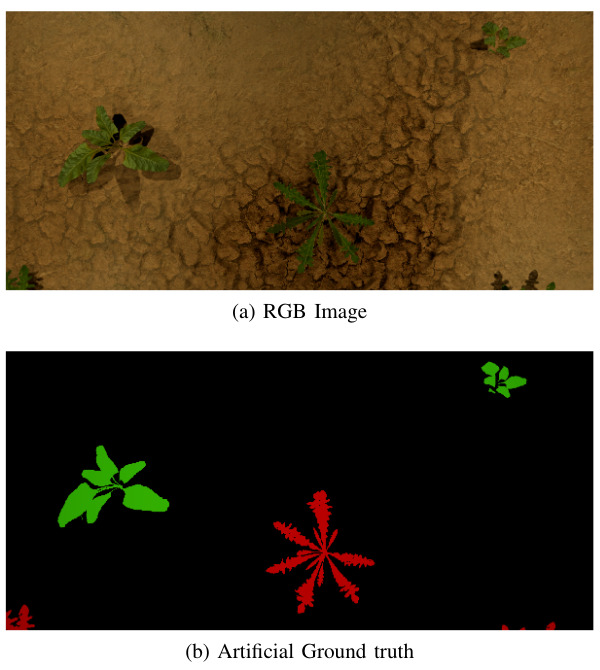
\includegraphics[width=0.48\textwidth]{src/img/reated-pics/weeds.jpg}
    \caption{Procedural Generation of Agricultural Plants using Unreal Engine 4 \cite{di2017automatic}}
    \label{fig:relatex-example-weeds}
\end{wrapfigure}


Using procedurally generated models, geometries and materials in synthetic video data ensures a high degree of data variance, with no two objects looking exactly the same. This is achieved through modeling a randomization of object attributes, in a highly controllable way.


Projects that make use of procedurally generated objects include generative models for agricultural plant models \cite{di2017automatic,barth2018data}, trees \cite{hewitt2017proceduralTrees}, volumetric clouds \cite{bengtsson2022efficient}, and even entire urban planning areas generated with probabilistic grammars\cite{kar2019meta}.

Other projects use physical modeling of light to procedurally re-interpret existing images to create highly realistic images from existing synthetic datasets \cite{tsirikoglou2017procedural,wrenninge2018synscapes}.

All game engines mentioned in Section \ref{sec:graphics-engines} have an implementation for procedural modeling. Unity has "Procedural Mesh Geometry"\footnote{\url{https://docs.unity3d.com/560/Documentation/Manual/GeneratingMeshGeometryProcedurally.html}} and "Procedural Materials" \footnote{\url{https://docs.unity3d.com/560/Documentation/Manual/ProceduralMaterials.html}}, Unreal has "Procedural Mesh" \footnote{\url{https://docs.unrealengine.com/4.26/en-US/BlueprintAPI/Components/ProceduralMesh/}}, and Blender has "Geometry Nodes" \footnote{\url{https://docs.blender.org/manual/en/latest/modeling/geometry_nodes/index.html}} and "Shader Nodes"\footnote{\url{https://docs.blender.org/manual/en/latest/render/shader_nodes/index.html}}. However, these features are not frequently used in synthetic data generation tasks to their fullest extent.

Use cases for procedural modeling with game engines are mentioned in the next section.

\section{Use Cases}
\label{sec:use-cases}

Procedural modeling can be used to construct synthetic datasets of any type of outdoor scene. It requires, however, some data describing the layout of a scene: road positions, terrain maps, and building profiles. These types of data can be found in large quantities in Geographic Information Systems (GIS), which contain satellite imagery for the whole planet, as well as accurate terrain and street map information.

A notable use of procedural modeling together with GIS data is the video game "Microsoft Flight Simulator 2020", which realistically models the entirety of Planet Earth at a scale of 1 to 1, complete with trillions of trees, dynamic weather systems and accurate renditions of all major cities around the globe \footnote{\url{https://www.pcgamesn.com/microsoft-flight-simulator/planet-earth-simulation}}.

\begin{figure}[H]
    \centering
    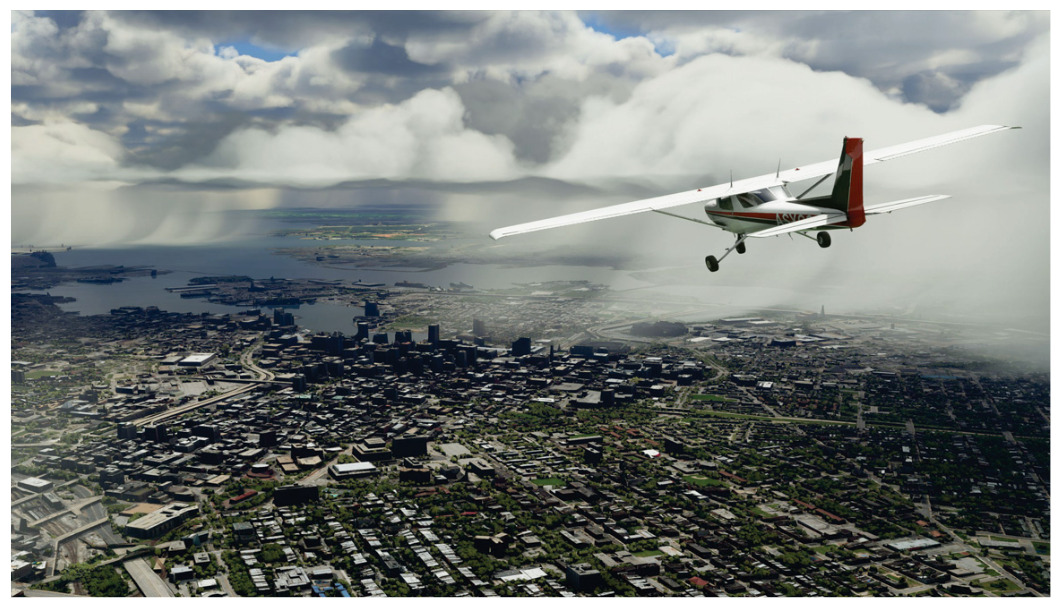
\includegraphics[width=\textwidth]{src/img/reated-pics/flight-sim.jpg}
    \caption{Screenshot from Microsoft Flight Simulator 2020, showing volumetric clouds and procedurally modeled cityscape \cite{bengtsson2022efficient}}
    \label{fig:relatex-example-msft}
\end{figure}

We propose combining GIS data with procedural modeling to obtain an outdoor scene generator with high data diversity and realistic graphics. While applications range from autonomous drone control to self-driving cars, we chose to focus our efforts on the problem of rail track semantic segmentation and anomaly detection.

The methodology used for building such a framework is outlined in Chapter \ref{chapter:approach}, and the actual implementation is explained in Chapter \ref{chapter:implementation}.